\newpage
\begin{Pro}
    Utiliza el algoritmo de simulación de NFA para simular los siguientes NFAs en la entrada aabb:
\end{Pro}

\begin{itemize}
    \item
    \begin{figure}[h!]
        \centering
        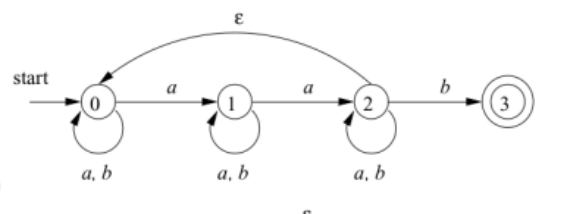
\includegraphics[width=0.5\textwidth]{images/8a.png}
        \caption{Automata Finito No Determinista, ejercicio 8 a}
    \end{figure}
    \begin{enumerate}
        \item Inicalizamos S con $\epsilon - closure (0)$ y $c$ con $a$ :
        \begin{align*}
            S &= \{0\} \\
            c &= a
        \end{align*}
        \item Calculamos $move(S, a)$, calculamos su cerradura asignamos el resultado a $S$ y actualizamos $c$ :
        \begin{align*}
            move(S, a) &= \{0, 1\} \\
            S &= \epsilon-closure (move(S, a)) = \{0, 1\} \\
            c &= a
        \end{align*}
        \item Es análogo al paso anterior:
        \begin{align*}
            move(S, a) &= \{0, 1, 2\} \\
            S &= \epsilon-closure (move(S, a)) = \{0, 1, 2\} \\
            c &= b
        \end{align*}
        \item Es análogo al paso anterior pero calculamos $move(S, b)$:
        \begin{align*}
            move(S, b) &= \{0, 1, 2, 3\} \\
            S &= \epsilon-closure (move(S, b)) = \{0, 1, 2, 3\} \\
            c &= b
        \end{align*}
        \item Es análogo al paso anterior:
        \begin{align*}
            move(S, b) &= \{0, 1, 2, 3\} \\
            S &= \epsilon-closure (move(S, b)) = \{0, 1, 2, 3, \} \\
            c &= eof
        \end{align*}
        \item Como $c = eof$ y $S$ contiene el estado de aceptación $3$, la cadena es aceptada.
    \end{enumerate}
    %%%%%%%%%%%
    %%%%%%%%%%%
    %%%%%%%%%%%
    %%%%%%%%%%%
    \newpage
    \item
    \begin{figure}[h!]
        \centering
        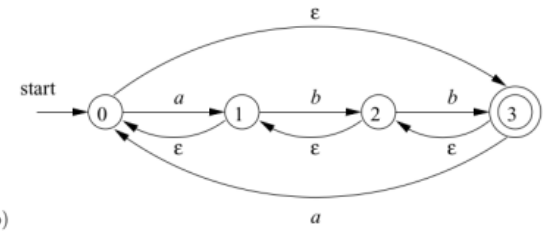
\includegraphics[width=0.5\textwidth]{images/8b.png}
        \caption{Automata Finito No Determinista, ejercicio 8 b}
    \end{figure}
    \begin{enumerate}
        \item Inicalizamos S con $\epsilon - closure (0)$ y $c$ con $a$ :
        \begin{align*}
            S &= \{0, 1, 2, 3\} \\
            c &= a
        \end{align*} 
        \item Calculamos $move(S, a)$, calculamos su cerradura asignamos el resultado a $S$ y actualizamos $c$ :
        \begin{align*}
            move(S, a) &= \{0, 1\} \\
            S &= \epsilon-closure (move(S, a)) = \{0, 1, 2, 3\} \\
            c &= a
        \end{align*}
        \item Es análogo al paso anterior:
        \begin{align*}
            move(S, a) &= \{0, 1\} \\
            S &= \epsilon-closure (move(S, a)) = \{0, 1, 2, 3\} \\
            c &= b
        \end{align*}
        \item Es análogo al paso anterior pero calculamos $move(S, b)$:
        \begin{align*}
            move(S, b) &= \{2, 3\} \\
            S &= \epsilon-closure (move(S, b)) = \{0, 1, 2, 3\} \\
            c &= b
        \end{align*}
        \item Es análogo al paso anterior:
        \begin{align*}
            move(S, b) &= \{2,3\} \\
            S &= \epsilon-closure (move(S, b)) = \{0, 1, 2, 3, \} \\
            c &= eof
        \end{align*}
        \item Como $c = eof$ y $S$ contiene el estado de aceptación $3$, la cadena es aceptada.
    \end{enumerate}

        
\end{itemize}
